% \introsection{Введение}

Как известно, вещество может находиться в трёх агрегатных состояниях~--- твёрдом,
жидком и газообразном, причём эти
состояния последовательно сменяются по мере возрастания температуры. Если~и
дальше нагревать газ, то сначала молекулы диссоциируют на атомы, а~затем и атомы
распадаются на электроны и ионы, так что газ становится \important{ионизованным},
представляя собой смесь из свободных электронов и ионов, а~также нейтральных
частиц. Если \term{степень ионизации} газа
(отношение числа ионизованных атомов к их полному числу) оказывается достаточно велика, то
такой газ может обладать качественно новыми свойствами.
Взаимодействие между заряженными частицами приобретает \important{коллективный} характер,
так что описание свойств среды не может быть сведено к обычному газу,
содержащему некоторое количество отдельных заряженных частиц.
Такое состояние ионизованного газа называется \term{плазмой}.
Плазму называют также четвёртым состоянием вещества.
Более точное определение этого понятия будет дано далее.

Из характерных свойств плазмы можно выделить высокую электропроводность и
\term{квазинейтральность}. Ввиду наличия большого числа свободных
заряженных частиц плазма, в противоположность нейтральному газу, сильно
взаимодействует с электрическим и магнитным полями.
При этом частицы в плазме стремятся распределиться в пространстве таким образом,
чтобы средняя плотность заряда была равна нулю. Равенство концентраций
положительных и отрицательных частиц нарушается, как правило,
лишь в микроскопических масштабах из-за тепловых флуктуаций.

Первое описание газовой плазмы дал И.~Ленгмюр (1923~г.), исследуя электрический
разряд в газе низкого давления (тлеющий разряд). Он назвал плазмой <<ярко
светящийся газ, состоящий из электронов, ионов разных сортов и нейтральных
атомов и молекул>>. Он же ввёл сам термин~--- плазма (от греческого глагола,
обозначающего <<разрыхляться>>, <<расползаться>>).
% ~--- и основные параметры,
% характеризующие плазму: плотности составляющих её частиц~--- электронов~---
% $n_e$, ионов~--- $n_i$, нейтральных частиц~--- $n_0$ и их температуры~---
% соответственно $T_e$, $T_i$,~$T_0$.

Свечение плазмы, являющееся следствием непрерывно идущей
рекомбинации электронов и ионов в нейтральные атомы, сопровождается выделением
энергии и уменьшением концентрации электронов и ионов. Стационарное состояние
плазмы может существовать лишь при наличии непрерывно действующего источника
энергии. Им может быть электрический разряд в газе (газоразрядная плазма),
происходящий в постоянном электрическом поле (обычный газовый разряд,
дуга и т.~д.) или в высокочастотном поле (индукционные катушки,
запитанные током высокой частоты электроды и т.~д.).
Плазма может образовываться и при термической ионизации газа, если газовая среда
поддерживается при достаточно высокой температуре (пламя газовой
горелки). Плазма образуется в фокальной области мощных лазерных установок и при
многих других условиях. Звёздная плазма существует за счёт выделения энергии
в реакциях ядерного синтеза.

Плазма исследуется также в связи с проблемой создания магнитогидродинамических
генераторов~--- преобразователей
механической энергии движущегося в магнитном поле проводящего газа в
электрическую энергию. Ещё одно важное направление использования плазмы~---
применение её для проведения химических реакций, которые в горячей
сильно ионизованной газовой среде происходят очень быстро и эффективно.
Большой интерес представляет плазма, существующая в атмосфере Земли и планет, а
также в космосе. Атмосферная плазма создаётся ультрафиолетовым излучением
Солнца. Электроны плазмы захватываются магнитным полем Земли (движутся вокруг и
вдоль силовых линий магнитного поля) и образуют радиационные пояса на
расстояниях тысяч километров от поверхности Земли. Широко известны также
плазменные проводящие слои Хевисайда, обеспечивающие дальнюю радиосвязь
на коротких волнах.

В низкотемпературной плазме ($T\lesssim 10^4$~К) степень ионизации плазмы
обычно невелика. Например, в тлеющем газовом разряде (люминесцентные лампы)
плотность электронов составляет $n_e\sim 10^9\;\text{см}^{-3}$,
а плотность нейтральных молекул $n_0\sim 10^{14}\;\text{см}^{-3}$.
Лишь внутри звёзд и в установках, используемых для исследования проблем,
связанных с управляемым термоядерным синтезом,
где температуры могут достигать значений $T \sim 10^{6}\;К$ и более,
доля атомов, находящихся в ионизированном состоянии, приближается
к единице (\important{полностью ионизованная плазма}).
% Мощность, подводимая к таким установкам, измеряется мегаваттами.

\begin{figure}[ht]
%     \psfragfig[width=1\textwidth]{Images/Chapter_5/v5_0}{%
%   \psfrag{x}[br]{\footnotesize $n$, см$^{-3}$}
%   \psfrag{y}{\footnotesize $T$, эВ}
%   \psfrag{a}[cr]{\footnotesize $10^{-2}$}
%   \psfrag{b}[cr]{\footnotesize $10^{-1}$}
%   \psfrag{c}[cr]{\footnotesize $1$}
%   \psfrag{d}[cr]{\footnotesize $10$}
%   \psfrag{e}[cr]{\footnotesize $10^{2}$}
%   \psfrag{f}[cr]{\footnotesize $10^{3}$}
%   \psfrag{g}[cr]{\footnotesize $10^{4}$}
%   \psfrag{h}[cr]{\footnotesize $10^{5}$}
%   \psfrag{A}[ct]{\footnotesize $1$}
%   \psfrag{B}[ct]{\footnotesize $10^{10}$}
%   \psfrag{C}[ct]{\footnotesize $10^{20}$}
%   \psfrag{D}[ct]{\footnotesize $10^{30}$}%
% }
    \centering
    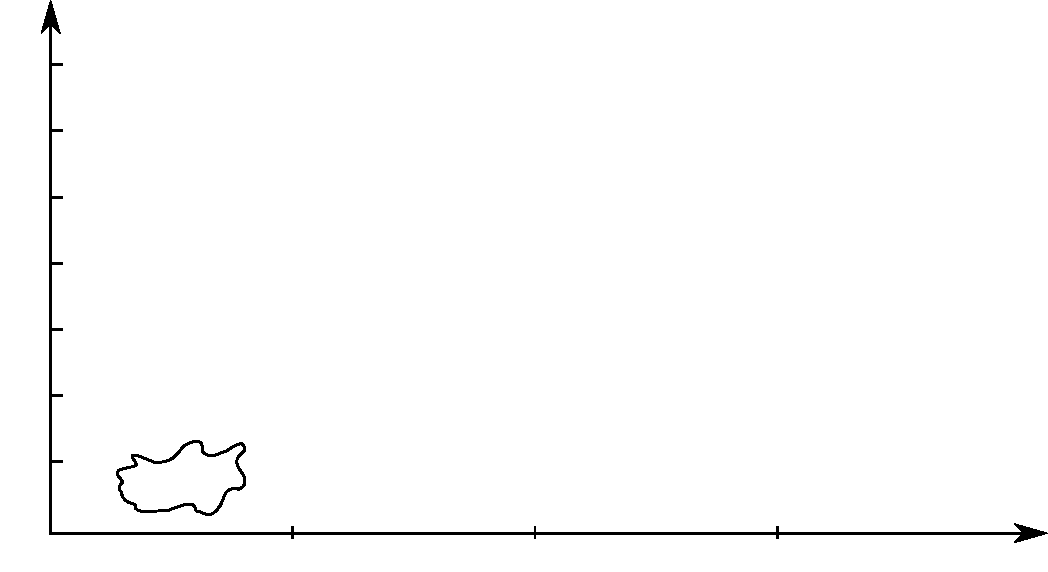
\includegraphics[width=0.95\textwidth]{Chapter_5/v5_0.pdf}
    \caption{Различные типы плазмы в лаборатории и природе. Температура
    дана в энергетических единицах ($1\;эВ\approx 11\,600\;К$)}
    \figmark{Types of plasma}
\end{figure}

Стационарное состояние плазмы может быть
\term{равновесным} или \term{неравновесным}.
В первом случае компоненты плазмы (электроны и ионы) имеют одну и ту же температуру,
а во втором~--- разную. При достаточно больших
давлениях (звёзды, пламя газовой горелки) между компонентами плазмы может
успевать установиться тепловое равновесие. При
малых давлениях ($\lambda\gtrsim d$, где $\lambda$~--- длина свободного пробега, а
$d$~--- характерный размер занятой
плазмой области) тепловое равновесие устанавливаться не успевает.
Так, в тлеющем газовом разряде мы обычно имеем дело с
<<горячими>> электронами и <<холодными>> ионами.
Электроны быстро ускоряются электрическим полем и почти не теряют
энергии при соударении с тяжёлыми ионами и атомами газа, а также при
столкновении со стенками газоразрядной трубки. Наоборот, ионы быстро отдают
полученную от поля энергию нейтральным атомам газа и атомам стенок, поскольку
массы их близки. В результате реализуются условия, при которых электроны
и ионы характеризуются разными температурами ($T_e > T_i$).

% Температура плазмы, как правило, измеряется не в градусах,
% а в эле-ктрон-вольтах ($1~\text{эВ}\approx 11\,600~\text{К}$). При расчётах
% плазменных явлений обычно используется система СГС.

Свойствами, характерными для газовой плазмы, обладают и некоторые другие среды,
называемые по этой причине
\important{плазмоподобными} средами, или просто плазмами: в этом смысле термин
\term{плазма} встречается в научной литературе во множественном числе.
В~качестве примеров различных плазм можно назвать плазму металлов,
электронно-дырочную плазму полупроводников, нуклонную плазму атомного ядра.
Различные типы плазм, встречающихся как в лабораторных условиях,
так и в природе, можно достаточно наглядно представить на плоскости параметров:
температура плазмы~--- плотность числа частиц (рис.~\figref{Types of plasma}).
% Под температурой плазмы в каждом конкретном случае понимают температуру тех
% заряженных частиц, которые определяют плазменные свойства рассматриваемой среды:
% в большинстве случаев это электроны.



\introsection{Основные свойства плазмы}
\label{sec:plasma}

Определяющими свойствами плазмы являются коллективный характер её движения
и квазинейтральность (равенство нулю средней плотности заряда).
Рассмотрим простейший вид коллективных плазменных колебаний. Здесь и далее
в этом разделе будем использовать систему СГС, как это принято в физике плазмы.

\begin{wrapfigure}{o}{0.4\textwidth}
% \psfragfig[width=0.3\textwidth]{Images/Chapter_5/v5_1}{%
%     \psfrag{E}[cb]{$E$}
%     \psfrag{0}[ct]{0}
%     \psfrag{X}{$X$}
%     \psfrag{x}[ct]{$x$}%
% }
    \centering
    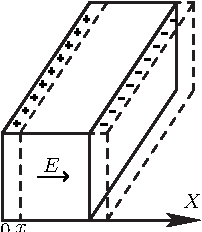
\includegraphics[width=0.3\textwidth]{Chapter_5/v5_1.pdf}
    \caption{Плазменные колебания}
    \figmark{1}
\end{wrapfigure}

\paragraph{Плазменная частота.}
Выделим в нейтральной плазме некоторый объём в виде параллелепипеда
(см. рис.~\figref{1}).
Обозначим концентрацию электронов как $n_e$; ионы для простоты будем считать
однозарядными ($Z=1$), тогда их концентрация такая же, как у электронов: $n_i=n_e$.
Предположим, что все электроны сместились на расстояние $x$ относительно ионов
(ионы как существенно более тяжёлые частицы можно считать неподвижными).
% (ионы занимают объём, изображённый сплошными, а электроны~--- пунктирными линиями).
В результате на боковых гранях параллелепипеда возникнут нескомпенсированные
поверхностные заряды с плотностью
\begin{equation*}
%     \eqmark{5.13}
    \sigma = \pm n_e e x.
\end{equation*}
Эти заряды --- как две пластины конденсатора --- создадут электрическое поле
\begin{equation*}
%     \eqmark{5.14}
    E=4\pi n_e e x.
\end{equation*}
В свою очередь это поле будет действовать на электроны,
придавая им ускорение, равное
\begin{equation*}
%     \eqmark{5.15}
    \frac{d^2x}{dt^2}=-\frac{eE}{m}=-\frac{4\pi ne^2}{m}x.
\end{equation*}
Видно, что полученное уравнение описывает гармонические колебания с частотой
\begin{equation}
    \eqmark{plasma-freq}
    \omega_p=\sqrt{\frac{4\pi n_e e^2}{m_e}}.
\end{equation}

Таким образом, мы получили частоту коллективных колебаний
электронов относительно квазинейтрального состояния. Такие колебания
называют \term{ленгмюровскими}, а частоту $\omega_p$ ---
\term{плазменной} или \term{ленгмюровской}. Эта частота ---
одна из важнейших характеристик плазмы.
Она задает естественный масштаб времени для плазмы: это~--- время
отклика на флуктуацию плотности заряда в плазме,
и определяет многие происходящие в ней процессы: от собственно плазменных
колебаний до распространения электромагнитных волн в ней.

% Для рассчётов можно использовать практическую формулу
% \begin{equation}
%     \eqmark{omegap-practical}
%  \omega_p =5,65\cdot10^4\sqrt{n[\text{см}^{-3}]}\;рад/с.
% \end{equation}

\paragraph{Дебаевский радиус.}
%  Учитывая это, дебаевский радиус экранирования можно интерпретировать
% следующим образом.
Плазменные колебания могут быть раскачены как с счёт внешнего воздействия
(например, при прохождении электромагнитной волны), так и за счёт
тепловой энергии, содержащейся непосредственно в плазме.
Оценим амплитуду колебаний электронов относительно ионов,
возникающих за счёт тепловых флуктуаций.

Пусть электроны колеблются с некоторой амплитудой $x_0$ и частотой $\omega_p$.
Тогда амплитуда их скорости равна $v_0 = \omega_p x_0$.
Полная энергия колебаний, как известно из механики,
равна максимальному значению кинетической энергии.
В расчёте на один электрон имеем энергию $W= \frac12 m_e \omega_p^2 x_0^2$.
С другой стороны, из термодинамики известно, что эта энергия должна
быть равна тепловой энергии, приходящейся на одну степень свободы
$W_Т = \frac12 \kB T_e$. Отсюда находим $x_0^2 = \frac{\kB T_e/m_e}{\omega_p^2}$.
Выразим с учётом \eqref{plasma-freq} амплитуду колебаний и обозначим полученный
результат как
\begin{equation}
    \eqmark{debye-rad}
    r_D=\sqrt{\frac{\kB T_e}{4\pi n_e e^2}}.
\end{equation}
Величину $r_D$ называют \term{дебаевским радиусом}
(или \term{дебаевской длиной}).
Это ещё один важный плазменный параметр, задающий характерный масштаб
многих плазменных явлений.

Видно, что дебаевская длина есть амплитуда ленгмюровских колебаний,
возбуждаемых тепловыми флуктуациями. Она задаёт масштаб, на котором возможно
\important{нарушение квазинейтральности} плазмы (в отсутствие внешнего поля).
Заметим также, что формулу \eqref{debye-rad} можно переписать как
\[
r_D = \frac{v_{Te}}{\omega_p},
\]
где $v_{Te}=\sqrt{\kB T_e/m_e}$~--- скорость, по порядку величины равная
средней тепловой скорости движения электронов.

Таким образом, плазменная частота $\omega_p$ и дебаевская длина $r_D$
есть две важнейшие характеристики плазмы, определяющие в том числе
временной и пространственный масштабы коллективного движения электронов
относительно ионов.

% Как следует из \eqref{plasma-freq}, плазменная частота определяется только плотностью
% электронов (и универсальными постоянными).
% Можно строго доказать, что она не зависит от формы рассматриваемого возмущения и
% является, таким образом,
% локальной характеристикой плазмы. Плазменная частота является не
% единственной~--- но важнейшей~--- характерной частотой
% плазмы. Она определяет коллективное движение электронов относительно ионов.

\paragraph{Плазменное экранирование.}
Рассмотрим ещё одну задачу, в которой дебаевская длина играет роль
ключевого параметра.

Поместим в плазму с температурой $T$ некоторую пробную частицу, имеющую фиксированный
положительный $+q$ и найдём, как распределятся плазменные частицы вокруг неё.
Будем считать, что частица достаточно массивна, так что её можно
считать неподвижной (в качестве такого пробного заряда можно рассмотреть
и один из ионов плазмы, поскольку $m_i \gg m_e$).

Заряд будет притягивать к себе плазменные электроны, в результате чего
вокруг него образуется отрицательно заряженная <<подушка>>,
\important{экранирующая} поле заряда на большом расстоянии от него ---
электрическое поле вокруг $q$ будет убывать с расстоянием $r$
не по закону $q/r^2$, а существенно быстрее.
Если бы электроны не имели кинетической энергии, то они так <<облепили>>
бы пробный заряд, что его собственное поле было бы полностью скомпенсировано.
Тепловое движение мешает такой компенсации.

\begin{wrapfigure}{o}{0.3\textwidth}
\centering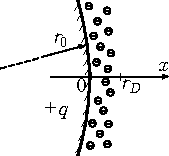
\includegraphics[width=\linewidth]{Chapter_5/v5-screen1.pdf}
\caption{Упрощенная геометрия задачи об экранировании заряда}
\end{wrapfigure}

Чтобы максимально наглядно выявить характерные особенности решения данной задачи,
предположим, что радиус $r_0$ пробной частицы велик (по сравнению с $r_D$)
и будем рассматривать распределение поля вблизи её поверхности ---
так мы сведём задачу к одномерной, сильно упростив выкладки, но не потеряв
качественные особенности решения.

% Как уже говорилось, во всяком сколько-нибудь большом объёме заряды ионов и электронов
% всегда практически компенсируют друг друга. Если хотя бы на некоторое
% время это оказывается не так, возникают сильные электрические поля,
% восстанавливающие квазинейтральность плазмы.
% Покажем, что именно дебаевская длина $r_D$ определяет размер области,
% внутри которой могут существовать заметные электрические
% поля и нарушаться квазинейтральность.

Пространственное распределение электронов в равновесии подчиняется
\important{закону Больцмана}:
\begin{equation}
    \eqmark{5.5}
    n_e=n_{e0} \cdot \exp\left(\frac{e\varphi}{\kB T}\right)
\end{equation}
Здесь $\varphi$~--- потенциал электростатического поля,
$n_{e0}$ --- концентрация электронов вдали от заряда, где $\varphi\to 0$.
Аналогичное соотношение можно записать и для ионов с заменой $-e\to e$
(по-прежнему считаем, что $Z=1$).
% \begin{equation}
%     \eqmark{5.5}
%     n_i(r) \approx n_0 \left(1-\frac{e\varphi}{\kB T}\right).
% \end{equation}
Будем считать, что температура электронов в плазме достаточно велика, так что
можно положить
\[
e\varphi\ll \kB T.
\]
Раскладывая больцмановскую экспоненту в ряд по этому малому параметру,
найдём объёмную плотность заряда в плазме:
\begin{equation}
\eqmark{rho_ei}
\rho = -en_e + en_i \approx -(n_{e0}+n_{i0}) \frac{e\varphi}{\kB T}.
\end{equation}

С другой стороны, распределение потенциала $\varphi$ в пространстве
однозначно связано с распределением плотности электрического заряда~$\rho$.
Применяя \important{теорему Гаусса} в дифференциальной форме
\[
\frac{dE}{dx}= 4\pi \rho,
\]
и пользуясь определением потенциала электростатического поля
$E = - \frac{d\varphi}{dx}$, получим
\begin{equation}
    \eqmark{poisson-1d}
    \frac{d^2\varphi}{dx^2} = - 4\pi \rho.
\end{equation}
Уравнение \eqref{poisson-1d} представляет собой частный (одномерный)
случай \important{уравнения Пуассона}.

Объединяя \eqref{poisson-1d} и \eqref{rho_ei}, получим окончательно
дифференциальное уравнение на потенциал поля $\varphi(x)$ вблизи пробной частицы:
\begin{equation}
    \frac{d^2\varphi}{dx^2} = \frac{\varphi}{r_D^2},
\end{equation}
где $r_D$ определяется соотношением \eqref{debye-rad}, в котором вместо
$n_e$ стоит полная концентрация частиц в плазме $n=n_{e0}+n_{i0}$.
Решение, удовлетворяющее граничным условиям
$\varphi(\infty)=0$ и~$\varphi(0)=\frac{q}{r_0}$, есть%
\footnote{Решая уравнение Пуассона в сферических координатах,
можно показать, что для точечного пробного заряда
(в том числе, для отдельного иона) распределение потенциала будет
\[
\varphi(r) = \frac{q}{r} e^{-\tfrac{r}{r_D}}.
\]}
\begin{equation}
\varphi(x) = \frac{q}{r_0} e^{-\tfrac{x}{r_D}}.
\end{equation}

\begin{wrapfigure}{o}{0.35\textwidth}
    \centering
    \import{Images/Chapter_5/}{v5-screen2.pdf_tex}
    \caption{Схематичное распределение потенциала (сплошная)
        и плазменных зарядов (пунктиры) и вблизи стороннего
        положительного заряда.}
\end{wrapfigure}

Таким образом, потенциал поля и его напряжённость,
а также концентрация плазменных частиц изменяются при удалении от
пробного заряда по экспоненциальному закону с характерной длиной порядка
дебаевского радиуса $r_D$. На расстояниях, превышающих $r_D$ в несколько раз,
плазму можно считать квазинейтральной, а поле заряда~$q$ практически
полностью экранированным. В связи с этим дебаевскую длину также называют
\term{радиусом экранирования}.

% Формула для дебаевского радиуса \eqref{5.10} не учитывает движение ионов.
В заключение отметим одно обстоятельство, часто вводящее в заблуждение.
В случае неравновесной плазмы, когда температуры электронов~$T_e$
и ионов~$T_i$ различны, можно определить две характерные длины --- для
электронов и ионов:
\[
r_{De} = \sqrt{\frac{\kB T_e}{4\pi n_e e^2}},
\qquad r_{Di} = \sqrt{\frac{\kB T_i}{4\pi n_i Z^2 e^2}}.
\]
Повторив изложенный выше вывод с учётом различия температур,
нетрудно получить (предлагаем проделать это самостоятельно)
радиус экранирования \important{стороннего заряда}:
\begin{equation}
\eqmark{debye-general}
r_{D} = \left(\frac{1}{r_{De}^2} + \frac{1}{r_{Di}^2}\right)^{-1/2}.
\end{equation}
% то есть вместо $T_e$ в формулу для дебаевского радиуса войдёт <<приведённая>>
% температура. В частности,
% при $T_e=T_i$ появляется множитель $\sqrt{2}$, а
Например, при $T_e\gg T_i$ (например, в плазме тлеющего газового разряда)
имеем $r_D\approx r_{Di}$, то есть радиус экранирования определяется
температурой холодных ионов~$T_i$.
При этом стоит подчеркнуть, что рассуждения предыдущего параграфа, сделанные
при выводе \eqref{debye-rad}, остаются в силе и при $T_e\gg T_i$:
масштаб, на котором нарушается квазинейтральность из-за тепловых
флуктуаций электронов относительно ионов, определяется именно значением
$r_{De}$, то есть зависит от температуры электронов~$T_e$.
% Чтобы разделить эти два не всегда сопадающие понятия,
% выражение \eqref{debye-rad} иногда
% называют \term{электронной поляризационной длиной}.

% формуле \eqref{5.10}
% вместо $T_e$ будет стоять~$T_i$.

% Подставляя \eqref{5.5} и \eqref{5.6} в \eqref{5.4}, получим:
% \begin{equation}
% 	\eqmark{5.7}
% 	\frac{d^2\varphi}{dr^2}+\frac{2}{r}\frac{d\varphi}{dr}=-4\pi
% ne\left[1-e^{e\varphi/\kB T_e}\right].
% \end{equation}
%
% Это уравнение нелинейно и в аналитическом виде не решается. Решение может быть
% найдено, если считать, что:
% \begin{equation}
% 	\eqmark{5.8}
% 	\frac{e\varphi}{\kB T_e}\ll1.
% \end{equation}
%
% В этом случае экспоненту можно разложить в ряд и уравнение \eqref{5.7}
% становится линейным:
% \begin{equation}
% 	\eqmark{5.9}
% \frac{d^2\varphi}{dr^2}+\frac{2}{r}\frac{d\varphi}{dr}=\frac{1}{r_D^2}\varphi,
% \end{equation}
% где введено обозначение
% \begin{equation}
% 	\eqmark{5.10}
% 	r_D=\sqrt{\frac{\kB T_e}{4\pi
% ne^2}}=743\sqrt{\frac{T_e~(\text{эВ})}{n~(\text{см}^{-3})}}~(\text{см}).
% \end{equation}

% Это решение правильно ведёт себя около иона (где $\varphi\propto e/r$) и
% обращается в нуль на бесконечности. Мы нашли,
% следовательно, искомое решение задачи. Оно показывает, что вследствие
% экранирующего действия электронов поле иона
% убывает с расстоянием экспоненциально с характерной длиной, равной $r_D$~---
% дебаевскому радиусу
% (сам Дебай ввёл понятие радиуса экранирования, рассматривая поле иона в
% электролите). В связи с этим дебаевскую длину также называют
% \import{радиусом экранирования}.

% Таким образом, плазму можно считать почти нейтральной (квазинейтральной)
% в областях, размеры которых существенно превосходят дебаевскую длину.
% При $T=10^4$~К ($\approx 1$~эВ) и $n=10^9 ~\text{см}^{-3}$, $r_D\approx
% 1,6\cdot10^{-2}$~см.

\paragraph{Идеальная и неидеальная плазма.}
Теперь можно дать \important{количественное} определение понятия плазма
(это определение также принадлежит Ленгмюру).

\term{Плазмой} называется \important{ионизованный газ, дебаевский радиус которого
    $r_D$ существенно меньше характерного размера области $a$, занимаемой этим газом}:
\begin{equation*}
	\sqrt{\frac{\kB T_e}{4\pi ne^2}}\ll a.
\end{equation*}

Именно при $a\gg r_D$ поведение среды носит существенно коллективный характер.
В противном случае среда может рассматриваться просто как газ
с примесью индивидуальных заряженных частиц.

Оценим энергию кулоновского взаимодействия частиц в плазме.
Как показано выше, распределение потенциала вокруг иона с зарядом~$q$
определяется законом экранирования
\[
\varphi = \frac{q}{r} e^{-r/r_D}.
\]
Вычитая потенциал самого иона $\varphi_0=\frac{q}{r}$, найдём
потенциал <<экранирующего облака>>. При $r\lesssim r_D$ имеем
\[
\varphi-\varphi_0 = \frac{q}{r}\left( e^{-r/r_D} - 1\right)
\approx - \frac{q}{r_D}.
\]
Воспользуемся известной формулой для электростатической энергии системы
зарядов $\varepsilon=\frac12 \sum_i \varphi_i q_i$, где $\varphi_i$ --- потенциал
в точке нахождения заряда $q_i$. Суммируя по всем ионам,
запишем плотность энергии взаимодействия зарядов в плазме:
\begin{equation}
w_{кул} \approx -\frac12 n \frac{q^2}{r_D}.
\end{equation}

Сравним полученную энергию с тепловой $w_T \sim n \kB T$:
\begin{equation}
\frac{w_T}{w_{кул}} \sim
\frac{\kB T r_D}{q^2} \sim 4\pi n r_D^3.
\end{equation}
Видно, что отношение тепловой и кулоновской энергии в плазме по порядку величины
есть число частиц в сфере радиуса $r_D$:
\begin{equation}N_D = \frac43 \pi n r_D^3.
\end{equation}


Плазму называют \term{идеальной}, если энергия кулоновского взаимодействия
мала по сравнению с тепловой, что выполняется, если число частиц
в <<дебаевской сфере>> велико, $N_D\gg 1$. Идеальная плазма во многом подобна
по своим свойствам идеальному газу. В неидеальной плазме ($N_D\lesssim 1$)
взаимодействие между частицами велико, так что она становится в некотором
смысле
подобна жидкости, а её описание значительно усложняется.

% Данный раздел имеет мало общего с реальностью. Длина свободного пробега
% электронов в плазме -- отдельный большой вопрос.
% Кроме того, данные формулы нигде не используются // ППВ

% \introsection{Электропроводность плазмы}
%
% Приложим к плазме электрическое поле с напряжённостью $\vec{E}$. Под его
% действием приходят в движение как электроны, так и
% ионы. Действующие на них силы мало отличаются друг от друга, а массы различаются
% очень сильно. Основными носителями тока
% являются поэтому электроны. Свободно двигаясь на пути свободного пробега,
% электроны приобретают направленную (дрейфовую)
% скорость. После очередного соударения скорость электрона может иметь самые
% разные направления, так что среднее значение
% этой скорости в начале пробега близко к нулю. В конце пробега оно равно
% \begin{equation*}
% 	\vec{v}_\text{кон}=-\frac{e\lambda}{m_e\average{v_e}}\vec{E},
% \end{equation*}
% где $\lambda$~--- длина свободного пробега, а $\average{v_e}$~--- тепловая
% скорость электрона, по сравнению с
% которой дрейфовая скорость обычно мала. Среднее значение дрейфовой скорости
% равно поэтому половине $v_\text{кон}$:
% \begin{equation}
% 	\eqmark{5.19}
% 	v_\text{др}=\frac{e\lambda E}{2m_e\average{v_e}}.
% \end{equation}
%
% Средняя тепловая скорость $\average{v_e}$ определяется из обычной формулы:
% \begin{equation}
% 	\eqmark{5.20}
% 	\average{v_e}=\sqrt{\frac{8\kB T_e}{\pi m_e}}.
% \end{equation}
%
% Объединяя эти формулы, найдём
% \begin{equation}
% 	\eqmark{5.21}
% 	\vec{v}_\text{др}=-b\vec{E},
% \end{equation}
% где подвижность электронов $b$ равна
% \begin{equation}
%  	\eqmark{5.22}
% 	b=\frac{e\lambda}{2\sqrt{\frac{8m_e}{\pi} \kB T_e}}.
% \end{equation}
%
% Электропроводность плазмы $\sigma$ определяется совместным дрейфовым движением
% всех электронов, так что
% \begin{equation}
% 	\eqmark{5.23}
% 	\sigma=\frac{j}{E}=\frac{n_eev_{др}}{E}=neb=\frac{e^2\lambda
% n_e}{2\sqrt{\frac{8m_e}{\pi} \kB T_ei}}.
% \end{equation}
%
% Полученная формула показывает, что электропроводность плазмы пропорциональна
% концентрации электронов и уменьшается с
% ростом температуры плазмы. Длина свободного пробега $\lambda$ в
% слабоионизированной плазме определяется не столько
% плотностью электронов $n_e$, сколько плотностью газа.

\introsection{Одиночный зонд}
\label{sec:single}

Одним из самых простых методов измерения свойств плазмы является измерение
электрического потенциала с помощью зондов~---
небольших проводников, вводимых в плазму.
% Как уже говорилось выше, метод зондов был разработан Ленгмюром в начале
% двадцатых годов XX века.

При внесении проводника в плазму, он подвергается <<бомбарировке>>
со стороны её заряженых частиц. Как известно из молекулярной физики,
число частиц, ударяющихся в идеальном газе в секунду о единичную поверхность,
равно
\begin{equation}
    \eqmark{nv4}
j = \frac14 n\overline{v},
\end{equation}
где $\overline{v} = \sqrt{\frac{8\kB T}{\pi m}}$ --- их средня тепловая скорость.
Поскольку $m_e \ll m_i$, тепловые скорости электронов, как правило, существенно
превосходят скорости ионов, поэтому в равновесии проводник зарядится отрицательно.
Отрицательный потенциал $-U_f$ (относительно плазмы),
до которого заряжается помещённый в неё зонд,
называют \term{плавающим}.

\begin{wrapfigure}{o}{0.5\textwidth}
%     \psfragfig[width=0.5\textwidth]{Images/Chapter_5/v5_8}{%
%     \psfrag{x}{$x$}
%     \psfrag{r}[tc]{$r_D$}
%     \psfrag{f}[rb]{$\varphi(x)$}
%     \psfrag{v}[cc]{$U_f$}%
% }
    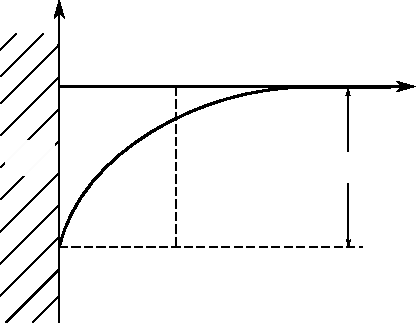
\includegraphics[width=0.5\textwidth]{Images/Chapter_5/v5_8.pdf}
    \caption{Распределение потенциала в~окрестности зонда}
    \figmark{Potential distribution}
\end{wrapfigure}

При плавающем потенциале количество попадающих на зонд ионов и электронов
уравнивается, так как до него могут доходить лишь наиболее быстрые
электроны и практически все ионы. Вокруг отрицательно заряженного зонда
образуется область положительного пространственного заряда,
экранирующего плазму от зонда (рис.~\figref{Potential distribution}),
размер которой порядка дебаевского радиуса.

За счёт теплового движения электронов и ионов
через зонд могут протекать токи, определяемые полным числом
движущихся в его сторону частиц. Пользуясь \eqref{nv4}, обозначим эти токи
как
\begin{equation}
    \eqmark{5.24}
    I_{e0}=\frac{n\overline{v}_e}{4}eS,\qquad
    I_{i0}=\frac{n\overline{v}_i}{4}eS,
\end{equation}
где $S$ --- площадь зонда, $n=n_e=n_i$. Эти токи также можно назвать
\term{тепловыми}.

Наличие отрицательного плавающего потенциала $-U_f$ на электроде практически
не влияет на ионный ток: $I_i \approx I_{i0}$. Электронный же ток
уменьшится, поскольку лишь часть электронов, летящих к зонду,
способна преодолеть потенциальный барьер. Согласно распределению Больцмана
\begin{equation}
    \eqmark{5.26}
    I_e=I_{e0}\exp\left(-\frac{eU_f}{\kB T_e}\right).
\end{equation}
Если суммарный ток в цепи зонда равен нулю,
то в равновесии токи компенсируются: $I_i=I_e$. Отсюда находим
величину плавающего потенциала:
\begin{equation}
\eqmark{5.27}
U_f=-\frac{\kB T_e}{e}\ln\frac{\overline{v}_e}{\overline{v}_i}=
-\frac12 \frac{\kB T_e}{e}\ln\frac{T_e m_i}{T_i m_e}.
\end{equation}

Например, в тлеющем газовом разряде
$\kB T_e\approx 1$~эВ, $\kB T_i\approx \frac{1}{40}$~эВ (комнатная температура).
Положим для оценки $m_i\sim 10^4m_e$. Тогда
$U_f \approx \frac{1 В}{2} \ln (40 \cdot 10^4) \approx 6,5\;В$.
% \begin{equation*}
%     \eqmark{5.28}
%     U_f%=\frac12\cdot 1~эВ\ln(40\.10^4)=
%     \approx 6,5~\text{В}.
% \end{equation*}


Формула \eqref{5.27} даёт правильную оценку, но с количественной
точки зрения её нельзя считать надёжной.
Во-первых существование <<дебаевского слоя>> вокруг зонда вносит некоторую
неопределённость в величину $S$. Если размер зонда значительно превышает
дебаевский радиус, это обстоятельство несущественно; однако если дебаевский
радиус велик, поправка может быть значимой.
Во вторых, при выводе было сделано плохо оправданное предположение,
что движение ионов у зонда близко к тепловому.
Это, конечно, справедливо вдали от дебаевского слоя зонда,
но не около него и тем более не в нём, где ионы подвергаются
ускоряющему действию довольно сильного электрического поля.
На практике требуется внести поправку в формулу ионного тока~$I_{i0}$.
% Тем не менее для грубых оценок \eqref{5.27} может быть использована.

\paragraph{Исследование плазмы с~помощью одиночных~зондов.}

При исследовании плазмы с помощью зондов на них подаются напряжения и
исследуются вольт-амперные
характеристики (ВАХ). Схема опытов изображена на \figref{Plasma study with
single probe}, на котором изображены два погружённых в плазму электрода и
источник $\mathcal{E}$, создающий между ними регулируемую разность потенциалов.
Пусть контактирующая с плазмой поверхность одного
электрода существенно меньше, чем у другого. Электрод с малой поверхностью будем
называть зондом, а электрод с большой
поверхностью~--- опорным электродом. Рассмотрим, как зависит ток $I_з$ в цепи
зонда от потенциала зонда~$U_з$
относительно опорного электрода.

\begin{figure}[h]
	\centering
%     \psfragfig[width=0.5\textwidth]{Images/Chapter_5/v5_9}{%
% 	\psfrag{I}[cc]{$I$}
%     \psfrag{U}[cc]{$U$}}
	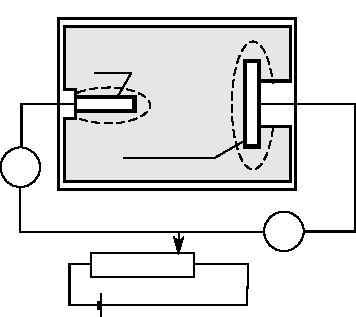
\includegraphics[width=0.5\textwidth]{Chapter_5/v5_9}
	\caption{Исследование плазмы с~помощью одиночного~зонда}
	\figmark{Plasma study with single probe}
\end{figure}

Рассмотрим вначале случай, когда разность потенциалов в плазме равна нулю.
Пусть потенциометр (рис.~\figref{Plasma study with single probe}) установлен
так, что зонд и опорный электрод соединены накоротко.
Ясно, что в этом случае они представляют собой один электрод сложной формы,
внесённый в плазму. Зарядившись отрицательно, они принимают относительно
плазмы потенциал $-U_f$. Полный ток на каждый электрод равен нулю, значит,
электронный ток равен ионному, $I_e=I_i$.

Если в плазме есть разность потенциалов $\Delta U$,
то ток зонда обращается в нуль, если потенциалы электродов
смещены на величины $U_f$ относительно исходных потенциалов
участков плазмы, в которые они погружены.
% Необходимая для этого разность потенциалов между зондом и опорным электродом
% равна разности потенциалов между соответствующими участками плазмы.
Таким образом, измеряя потенциал зонда относительно опорного электрода при нулевом
токе, можно исследовать распределение потенциала в плазме.

Сведения о температуре и плотности зарядов в плазме получают, снимая
вольт-амперную характеристику зонда.
При изменении потенциала зонда $U_з$ через плазму и по внешней цепи
начинает проходить ток, так как баланс между электронным и ионным током на зонд
нарушается. При этом токи, проходящие через зонд и опорный электрод, конечно,
равны друг другу, а плотности тока различны, так как площади
электродов существенно различаются.
Плотность тока, идущего через опорный электрод, из-за большой площади последнего
всегда очень мала, и, следовательно, его потенциал относительно плазмы
практически всегда равен $-U_f$. При небольшом размере зонда наибольшая
плотность тока возникает около него, так что практически всё падение напряжения
приходится на дебаевский слой, окружающий зонд.

Для эквипотенциальной плазмы зависимость зондового тока $I_\text{з}$
от потенциала зонда $U_\text{з}$ имеет вид, показанный на рис.~\figref{Single probe VAC}.
Эта кривая носит название \term{зондовой характеристики}.

\begin{figure}[h]
%     \psfragfig[width=0.5\textwidth]{Images/Chapter_5/v5_10}{%
%     \psfrag{U}{$U_з$}
%     \psfrag{I}[br]{$I_з$}
%     \psfrag{0}[br]{0}
%     \psfrag{a}[cr]{$I_{eн}-I_{iн}$}
%     \psfrag{b}[cr]{$I_{eн}$}
%     \psfrag{c}[cl]{$-I_{iн}$}
%     \psfrag{d}[tc]{$U_f$}
%     \psfrag{A}[rb]{$A$}}
    \centering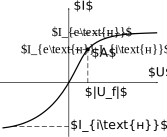
\includegraphics[width=0.5\textwidth]{Chapter_5/v5_10}
    \caption{Вольт-амперная характеристика одиночного~зонда}
    \figmark{Single probe VAC}
\end{figure}

На \important{левой ветви} характеристики (при $U_\text{з}<0$) весь ионный ток,
приходящий на границу дебаевского слоя, достигает зонда.
Ионный ток равен, следовательно, своему максимальному значению ---
\important{ионному току насыщения}~$I_{iн}$.
Электронный ток $I_e$ при смещении потенциала в сторону отрицательных
значений уменьшается и в пределе $U\to -\infty$ прекращается, $I_e\to 0$.
Отметим, что, хотя на первый взгляд, величина ионного тока
насыщения не должна зависеть от потенциала зонда ($I_{iн}=\const$),
на самом деле это не так. Дело в том, что при изменении потенциала
% во-первых, изменяется площадь поверхности дебаевского слоя и, во-вторых,
изменяются скорости ионов, которые быстро увеличиваются при подлёте иона к электроду~---
от тепловых значений до значений, определяемых величиной потенциала (см.
ниже формулу \eqref{5.31}).
Поэтому при дальнейшем сдвиге потенциала зонда в сторону отрицательных значений
ток зонда возрастает, хотя и не очень сильно.

На правой ветви характеристики (при $U_\text{з}>0$) потенциал зонда превышает
потенциал опорного электрода, но вначале (вплоть до точки~$A$)
остаётся ниже потенциала плазмы. При этом ионный ток на зонд
практически не меняется ($I_i\approx I_{iн}$),
а электронный ток возрастает. В точке~$A$~--- при~$U_\text{з}=U_f$~---
слой пространственного заряда (дебаевский слой) исчезает и оба тока~---
электронный и ионный~--- подходят к зонду беспрепятственно.
% При этом электронный ток существенно превосходит ионный, $I_e\gg I_i$,
% поскольку плотности электронов
% и ионов близки друг к другу, а тепловые скорости существенно различаются
% ($n_i=n_e$, $\overline{v}_e\gg \overline{v}_i$).

При дальнейшем увеличении~$U_з$ ионный ток подавляется, а ток электронов
достигает насыщения $I\approx I_{eн}$
(при этом на самом деле ток насыщения медленно возрастает по тем же причинам,
по которым изменяется ионный ток насыщения при $U_з < 0$).

Участок характеристики, расположенный влево от точки $A$, носит название
\term{ионной} ветви (ионный ток равен току
насыщения), а участок вправо от точки $A$ называется \term{электронной}
ветвью вольт-амперной характеристики (электронный ток равен току насыщения).

Электронный ток насыщения может быть оценен по формуле
\eqref{5.24}, $I_{eн}\approx I_{e0}$. При этом для ионного тока
аналогичная оценка оказывается слишком груба ---
как уже упоминалось, скорости ионов вблизи зонда
определяются не температурой плазмы, а разностью потенциалов между плазмой и
зондом:
\begin{equation*}
	\eqmark{5.30}
	v_i\approx\sqrt{\frac{2eU}{m_i}}.
\end{equation*}
В связи с этим для вычисления этого тока лучше применять
полуэмпирическую формулу, предложенную Бомом:
\begin{equation}
	\eqmark{5.31}
	I_{i\text{н}}\approx 0,4 n_i eS\sqrt{\frac{2\kB T_e}{m_i}}.
\end{equation}
Структуру этой формулы нетрудно понять, замечая, что, согласно формуле
\eqref{5.27}, $U_f$ пропорционально $T_e$ (логарифмической
зависимостью $U_f$ при оценках следует пренебрегать).
% Численный коэффициент в формуле \eqref{5.31} требует более подробных расчётов.

В заключение заметим, что вид выражения \eqref{5.31}, в которое входят температура электронов и масса
ионов, характерна для многих явлений в плазме.
Внешние поля приводят к быстрому перемещению электронов и к существенно более
медленному движению ионов. Значительное
перемещение электронов относительно ионов, однако, невозможно, так как оно
нарушило бы квазинейтральность плазмы.
Движение плазмы определяется поэтому массой ионов. В то же время перемещение
электронов существенно зависит как от
приложенных полей, так и от электронной температуры. Процессы, которые
определяются параметрами, одни из которых
характерны для электронов (в нашем случае~$T_e$), а другие~--- для ионов (в
рассматриваемой формуле~--- $m_i$), обычно называются \term{амбиполярными}.

% При измерениях с помощью одиночного зонда в качестве опорного электрода часто
% используется анод газоразрядной трубки. Мы
% уже отмечали, что падение напряжения в положительном столбе разряда невелико,
% поэтому разности потенциалов, возникающие
% между анодом и зондом, также оказываются небольшими и легко доступны измерениям.
% Одиночные зонды используются для
% исследования распределения потенциала в плазме, для измерения электронной
% температуры и плотности электронов. Ещё лучше
% делать это с помощью двойных зондов.

\introsection{Двойной зонд}
\label{sec:double}

Двойным зондом называется система, состоящая из двух одинаковых зондов,
расположенных на небольшом расстоянии друг от
друга. Между зондами создаётся разность потенциалов~$U$, которая по величине много
меньше плавающего потенциала $U_f$, $|U|\ll U_f$. При
этом оба зонда имеют относительно плазмы близкий к плавающему отрицательный
потенциал, т.~е. находятся на \important{ионной} ветви
вольт-амперной характеристики (см. выше).

При отсутствии разности потенциалов ток между зондами равен нулю. Рассчитаем
величину тока, проходящего через двойной
зонд вблизи точки $I=0$. При небольших разностях потенциалов ионные токи на оба
зонда равны ионному току насыщения и
компенсируют друг друга. Величина результирующего тока целиком связана с
различием в электронных токах. Пусть потенциал
на первом зонде равен
\begin{equation}
	\eqmark{5.32}
	U_1=-U_f+\Delta U_1,
\end{equation}
а на втором
\begin{equation}
	\eqmark{5.33}
	U_2=-U_f+\Delta U_2.
\end{equation}

По предположению $\Delta U_1, \Delta U_2 \ll U_f$.
Напряжение $U$ между зондами равно
\begin{equation}
	\eqmark{5.34}
	U=U_2-U_1=\Delta U_2-\Delta U_1.
\end{equation}

Найдём ток, приходящий на первый электрод:
\begin{equation*}
	\begin{gathered}
        I_1=I_{i\text{н}}+I_{e1}=I_{i\text{н}}-I_{e0}
\exp\left(\frac{e(-U_f+\Delta U_1)}{\kB T_e}\right)=  \\
	 	=
        I_{i\text{н}}-\left[I_{e0}\exp\left(-\frac{eU_f}{\kB T_e}\right)\right]
\exp\left(\frac{e\Delta U_1} {\kB T_e} \right).
	\end{gathered}
\end{equation*}
Заметим, что при $\Delta U_1=0$ (при $U_1=U_f$) электронный и ионный ток
компенсируют друг друга. Это означает, что
заключённый в квадратные скобки множитель равен $I_{i\text{н}}$. Имеем поэтому
\begin{equation}
	\eqmark{5.35}
	I_1=I_{i\text{н}}\left[1-\exp\left(\frac{e\Delta U_1}{\kB T_e}\right)\right].
\end{equation}

Аналогично для второго электрода
\begin{equation}
	\eqmark{5.36}
	I_2=I_{i\text{н}}\left[1-\exp\left(\frac{e\Delta U_2}{\kB T_e}\right)\right].
\end{equation}

Заметим, что зонды 1 и 2 соединены \important{последовательно}~--- через плазму~---
и через них проходит один и тот же ток $I$, но в \important{разном} направлении.
Положим $I_1=-I_2=I$.
Выразим $\Delta U_1$ и $\Delta U_2$ из \eqref{5.35} и \eqref{5.36}:
\begin{equation*}
	\eqmark{5.38}
	\Delta U_1=\frac{\kB T_e}{e}\ln\left(1-\frac{I}{I_{i\text{н}}}\right),
\end{equation*}
\begin{equation*}
	\eqmark{5.39}
	\Delta U_2=\frac{\kB T_e}{e}\ln\left(1+\frac{I}{I_{i\text{н}}}\right).
\end{equation*}
Наконец, вычитая второе равенство из первого, найдём
\begin{equation*}
 	\eqmark{5.40}
	U=\Delta U_1-\Delta
U_2=\frac{\kB T_e}{e}\ln\frac{1-I/I_{i\text{н}}}{1+I/I_{i\text{н}}},
\end{equation*}
и разрешая это равенство относительно $I$, получим
\begin{equation}
	\eqmark{5.41}
	I=I_{i\text{н}}\th\frac{eU}{2\kB T_e}.
\end{equation}
Эта формула может служить для определения температуры электронов по форме
вольт-амперной характеристики двойного зонда.

Наблюдаемая на опыте зависимость тока от напряжения изображена на
рис.~\figref{Double probe VAC}. Заметим, что
эта кривая отличается от \eqref{5.41} существованием наклона у асимптот
в области больших $|U|$ (см. обсуждение тока насыщения в предыдущем параграфе).
% Наклон асимптот в первом приближении является линейным.
% Поэтому вместо \eqref{5.41} лучше писать
% \begin{equation}
% 	\eqmark{5.42}
% 	I=I_{i\text{н}}\th\frac{eU}{2\kB T_e}+aU,
% \end{equation}
% где $a$~--- некоторая константа, величина которой может быть найдена из опыта.

\begin{wrapfigure}{o}{0.5\textwidth}
%     \psfragfig[width=0.5\textwidth]{Images/Chapter_5/v5_11}{%
% 	\psfrag{U}{$U$}
% 	\psfrag{I}{$I$}
% 	\psfrag{0}[br]{0}
% 	\psfrag{1}[cr]{$I_{iн}$}
%     \psfrag{2}[cl]{$-I_{iн}$}}
	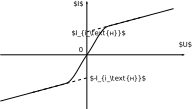
\includegraphics[width=0.5\textwidth]{Chapter_5/v5_11}
	\caption{Вольт-амперная характеристика двойного зонда}
	\figmark{Double probe VAC}
\end{wrapfigure}

Графики типа рис.~\figref{Double probe VAC} проще всего обрабатывать следующим
образом. Сначала находится $I_{i\text{н}}$ из пересечения асимптот
с осью $U=0$.
% Затем, по наклону асимптот, находится величина $a$.
После этого из \eqref{5.41} нетрудно определить $T_e$.
Дифференцируя эту формулу по $U$ в точке $U=0$ и принимая во внимание, что при
малых аргументах $\th x\approx x$,
% а при малых наклонах кривой насыщения $a\to 0$,
найдём
\begin{equation}
	\eqmark{5.43}
	\kB T_e=\frac12\frac{eI_{i\text{н}}}{\left.\frac{dI}{dU}\right|_{U=0}},
\end{equation}
где $\left.\frac{dI}{dU}\right|_{U=0}$ --- наклон характеристики зонда вблизи
начала координат. По известным $T_e$ и $I_{iн}$
можно из формулы \eqref{5.31} найти концентрацию плазмы $n$.

Таким образом,
двойные зонды удобно применять для измерения электронной температуры
и концентрации частиц в плазме.
